\documentclass[12pt, titlepage]{article}
\usepackage{booktabs}
\usepackage{tabularx}
\usepackage{hyperref}
\usepackage{graphicx}				
\usepackage{amssymb, amsmath}
\usepackage{enumerate}
\usepackage{mdframed}
\usepackage{float}
\usepackage{soul}
\usepackage{color}

\hypersetup{
    colorlinks,
    citecolor=black,
    filecolor=black,
    linkcolor=red,
    urlcolor=blue
}
\usepackage[round]{natbib}
\title{SE 3XA3: Software Requirements Specification\\PineSweeper}
\author{Team 07, PineApple
		\\ Prince Sandhu; sandhps2.
		\\ Varun Rathore; rathorvs.
		\\ Vishesh Gulatee; gulatev.
}
\date{\today}
\begin{document}
\maketitle
\pagenumbering{roman}
\tableofcontents
\newmdenv[linecolor=black]{reqbox}
\listoftables
\listoffigures
\setlength{\parindent}{0pt}
\begin{table}[bp]
\caption{\bf Revision History}
\begin{tabularx}{\textwidth}{p{3cm}p{2cm}X}
\toprule {\bf Date} & {\bf Version} & {\bf Notes}\\
\midrule
October 03 & 1.0 & Functional Requirements\\
October 04 & 1.1 & Completed Functional Requirements\\
October 07 & 1.2 &  Non-Functional Requirements\\
October 08 & 1.3 & Completed Non-Functional Requirements\\
October 09 & 1.4 & Project Drivers\\
October 11 & 1.5 & Completed Project Issues\\
October 11 & 1.6 & Completed LaTeX File\\
December 3 & 2.0 & Revision 1 \\

\bottomrule
\end{tabularx}
\end{table}
\newpage
\pagenumbering{arabic}

\section{Project Drivers}

\subsection{The Purpose of the Project}
The fundamental purpose of video games are to relieve a wide demographic of the public from boredom and stress. Over the past two
decades, the evolution of the video game development process and the technology involved, has ushered in a different focus and style
of video games. While these games provide users with a stunning visual experience, the model and gameplay have become
progressively complex. In an attempt to add realism, game developers have created games that when played, feel more like
accomplishing a stressful task that involves a steep learning curve. Users (gamers) are forced to clock in hours of their time, in order to
be able to play the game efficiently. Hence, individuals who are naturally skilled or put in said time and effort are rewarded. While this
may not seem to be a very serious problem, it defeats said fundamental purpose of the product. Additionally, games that do not follow
this trend have become obsolete and underappreciated. One such example is the once popular classic video game Minesweeper. To
that end, members of \textit{PineApple} attempt to redevelop Microsoft's beloved puzzle game as \textit{PineSweeper}, with the intention
of reintroducing the concept of challenging, yet simple video games to the masses, an intention that is shared by our client.

\subsection{The Stakeholders}
As mentioned, the primary goal of the project is to recreate the Minesweeper application that faithfully adapts the model, logic and rules
of the original game. To emphasize the project commitment in producing an application that can be played by any individual. Java
programming language will be used to create an application that can be used across a variety of operating systems. To add to the
applications appeal, the video game will feature a modern aesthetic feel and will give significance to user preference. As a play on the
team's name and to avoid using symbols or icons that may be received poorly by users, the mines in the game will be replace by
\textit{PineMines}, hence the name \textit{PineSweeper}.

\subsubsection{The Client}
The client of this project is \textit{McMaster University} and the project is commissioned by Professor \textit{Spencer Smith} of the university, who along with being in charge of oversight and providing guidance to team \textit{PineApple} throughout the design process, will be reviewing the final product prior to its deployment to the public.

\subsubsection{The Customers}
The application is designed to be used by members of the general public and avid gamers, of ages 7 and upwards. The consumer base
is not required to possess relevant knowledge or background regarding the logic and rules of the gameplay. The customer's role is
significant in the testing and validation phases, of  the design process.

\subsubsection{Other Stakeholders}
Other stakeholders include:
\begin{itemize}
	\item Members of team \textit{PineApple}, who are involved in the design, development and implementation of the project.
	\item The developer of \textit{JSweeper}, the open source implementation used as reference.
	\item Other independent game developers with similar aspirations and intentions.
\end{itemize}

\newpage
\subsection{Mandated Constraints}
\subsubsection{Solution Constraints}
The product shall operate using OS such as Windows, Linux and  Mac OS
Rationale: Clients and users use these conventional operating systems on their PC.
Fit Criterion: The final product will be tested in machines running the mentioned OS.

\subsubsection{Partner or Collaborative Applications}
The application is being re-developed based off a previous imitation of the Minesweeper game, developed in Java called
\textit{JSweeper}. Additionally, for the execution of the final product, system will require JRE, which will be integrated into 
the executable file.

\subsubsection{Schedule Constraints}
The product must be completed by 28th November, 2016, which is the last week of November, 2016.

\subsubsection{Budget Constraints}
To meet the requirements of the project, no funding is required and hence, the budget is non applicable.

\subsubsection{Enterprise Constraints}
The finished video game will be free to play and will be downloadable via the \textit{PineSweeper} Gitlab page.

\newpage
\subsection{Naming Conventions and Terminology}
\begin{enumerate}
	\item \textbf{AI}: Artificial Intelligence, a virtual machine's ability to mimic cognitive functions, most often 
	associated with humans (such as planning and perception).
	\item \textbf{API}: Application Program Interface. An API is a document that specifies the operation of library functions
	(methods in Java) used in a software application.
	\item \textbf{exe}: Executable file. A type of file that contains a program, that can be executed or run as 
	program in a computer.
	\item \textbf{Game mode}: Term used to indicate the game's difficulty level (beginner, intermediate and 						 advanced), as selected by the user.
	\item \textbf{Gameplay}: The interaction between a physical user and the video game's AI.
	\item \textbf{Gamers}: Common terminology used for users of video games.
	\item \textbf{GUI}: Graphical User Interface. Allows user to interact with the system, with the aid of visual 
	and graphical indicators.
	\item \textbf{JAR}: Java Archive. File format that compresses class files and resources of a project into one file.
	\item \textbf{JRE}: Java Runtime Environment. Tools required to develop and run java applications.
	\item \textbf{Mouse Click}: User input.
	\item \textbf{MVC}: Model-View-Controller software framework.
	\item \textbf{OS}: Operating System. System software that provides an environment for other programs.
	\item \textbf{PC}: Personal computer.
	\item \textbf{Flagged Cell}: a cell, whose contents are still hidden, but have been marked with a flag, 						 using the right click button of a mouse. The flag states that there is potentially a mine hidden.
	\item \textbf{\textit{PineMine}}: Rather than using a mine, which may invoke an aggressive response, the game 
	substitutes them with \textit{PineMines}, which also ties in the company's name.
\end{enumerate}

\vspace{10mm}

\subsection{Relevant Facts and Assumptions}
\subsubsection{Relevant Facts}
\begin{itemize}
	\item The original implementation used as reference had roughly blank lines of code. It has standard 
	license for open source and is executed as a java executable.
	\item The open-source project that the application is based upon has undocumented code, which needs 
	to be addressed during the reimplementation.
	\item The windows application is no longer a default application of the Windows OS. Instead it is a free 
	application with advertisements, downloadable from the windows store.
\end{itemize}

\subsubsection{Assumptions}
\begin{itemize}
	\item It is assumed that people like to play video games in their spare time, when they are bored and 
	when they are stressed out.
	\item It is assumed that gamers are looking for challenging yet simple to learn games.
\end{itemize}

\newpage
\section{Functional Requirements}

\subsection{The Scope of the Work and the Product}

\subsubsection{The Context of the Work}

\begin{figure}[!h]
	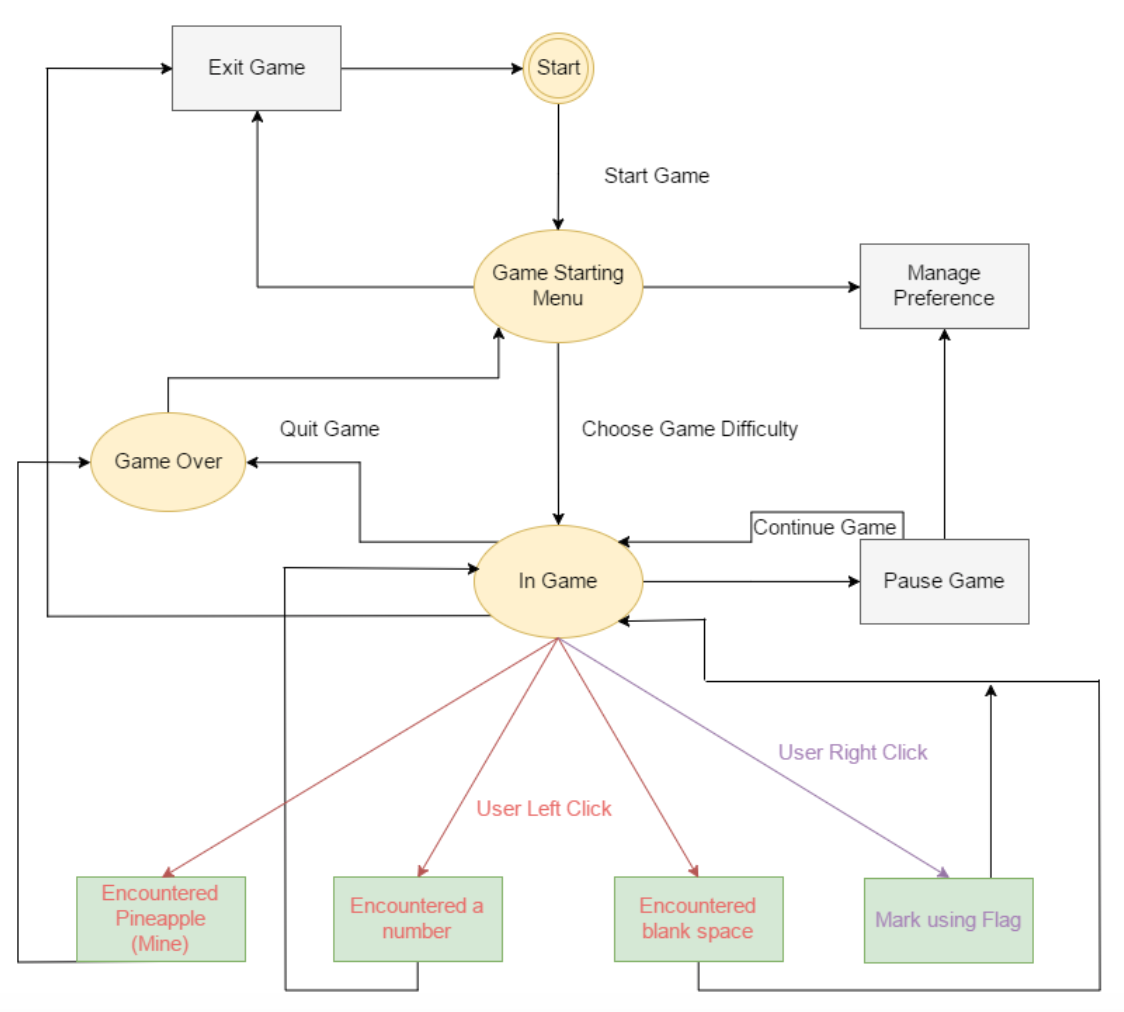
\includegraphics[width=\linewidth] {ContextFSM.png}
	\caption{Context Diagram}
\end{figure}

\subsubsection{Work Partitioning}
\begin{table}[H]
	\begin{tabularx}{\textwidth}{|X|X|X|}
\hline
		\textbf{Event Name} & \textbf{Input/Output} & \textbf{Summary} \\ 
		\hline
			User selects game difficulty. &
			Dimensions(IN)
			Graphical representation of game board (OUT) & 
			User selects difficulty, and the system generates the corresponding board size and number of hidden
			\textit{PineMines}. \\
		\hline
			User commences the game. &
			Dimensions(IN)
			Elapsed time starts (OUT) & 
			The user starts the game by pressing the a random cell within the game. As a result, the elapsed time starts. \\
		\hline
			User clicks on a cell that is not a \textit{PineMine}. &
			Mouse click (IN)
			Blank cell or numbered cell (OUT)
			Elapsed time continues (OUT) & 
			The user left-clicks on a covered cell, which is either a blank cell or a cell that contains a number. 
			The system uncovers the cell, the elapsed time and game proceed. \\
		\hline
			User marks a cell with a flag. &
			Mouse right click (IN)
			Flagged cell (OUT)
			Elapsed time continues (OUT) &
			The user right-clicks on a covered cell. The system marks the cell with a flag, the elapsed time 
			and the game proceed. \\
		\hline
			User clicks on a cell that is a \textit{PineMine}. &		
			Mouse right click (IN)
			\textit{PineMine} cell (OUT) &
			The user left-clicks on the pause game button. The game's elapsed time pauses, and 
			prevents the user from clicking on any cells until the resume game button has been clicked upon. \\
		\hline
			User resumes the game. &
			Mouse click (IN)
			Elapsed time continues (OUT) &
			The user left-clicks on the resume game button. The game's elapsed time resumes, and the game proceeds. \\
		\hline
	\end{tabularx}
		\caption{Work Partitioning}
		\label{Table}
\end{table}

\subsubsection{Individual Product Use Cases}

\begin{figure}[!h]
	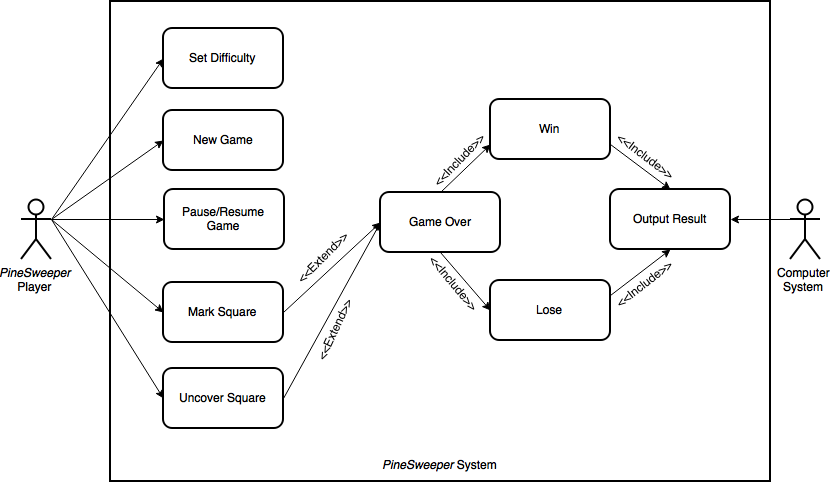
\includegraphics[width=\linewidth] {UseCase.png}
	\caption{Use Case Diagram}
\end{figure}

\newpage
\subsection{Functional Requirements}

\begin{reqbox}

\begin{tabular}{lll}
Requirement \#: 1 & Requirement Type: 2 & Event/Use case \#: \\
\end{tabular} \\

\textbf{Description}:  The system must allow the user to select from one of three game difficulties:
			         beginner, intermediate, and advanced. \\ \\
\textbf{Rationale}: Gives the user the option to change difficulties to suit their needs. As the difficulty
			     level increases, the corresponding board size and the number of mines increases.\\ \\
\textbf{Originator}: Prince Sandhu \\
\textbf{Fit Criterion}: In-game menu allows the user to change difficulty.\\

\begin{tabular}{ll}
\textbf{Customer Satisfaction}: 5 & \textbf{Customer Dissatisfaction}: 5 \\
\end{tabular}

\begin{tabular}{lll}
\textbf{Priority}: High & \textbf{Conflicts}: None & \textbf{Supporting Materials}: None \\
\end{tabular}

\begin{tabular}{l}
\textbf{History}: Created October 3, 2016.\\ \\
\end{tabular}

\end{reqbox}
% --------------------------------------------------------------------------------------------------------------------------------------------
\begin{reqbox}

\begin{tabular}{lll}
Requirement \#: 2 & Requirement Type: 2 & Event/Use case \#: \\
\end{tabular} \\

\textbf{Description}: The product shall be displayed using an N x M rectangular grid using the graphical user interface. \\ \\
\textbf{Rationale}: This step serves as a skeleton of the game board. It is necessary to have the board for the remaining
functions of the product.\\ \\
\textbf{Originator}: Prince Sandhu \\
\textbf{Fit Criterion}: Game grid is displayed at all times during gameplay.\\

\begin{tabular}{ll}
\textbf{Customer Satisfaction}: 5 & \textbf{Customer Dissatisfaction}: 5 \\
\end{tabular}

\begin{tabular}{lll}
\textbf{Priority}: High & \textbf{Conflicts}: None & \textbf{Supporting Materials}: None \\
\end{tabular}

\begin{tabular}{l}
\textbf{History}: Created October 3, 2016.\\ \\
\end{tabular}

\end{reqbox}
% --------------------------------------------------------------------------------------------------------------------------------------------
\begin{reqbox}

\begin{tabular}{lll}
Requirement \#: 3 & Requirement Type: 2 & Event/Use case \#: \\
\end{tabular} \\

\textbf{Description}: The contents of the hidden cell must be displayed when clicked upon. \\ \\
\textbf{Rationale}: A fundamental rule of MineSweeper; the game cannot be played without this 					    requirement.\\ \\
\textbf{Originator}: Prince Sandhu \\
\textbf{Fit Criterion}: A click uncovers the specified cell.\\

\begin{tabular}{ll}
\textbf{Customer Satisfaction}: 5 & \textbf{Customer Dissatisfaction}: 5 \\
\end{tabular}

\begin{tabular}{lll}
\textbf{Priority}: High & \textbf{Conflicts}: None & \textbf{Supporting Materials}: None \\
\end{tabular}

\begin{tabular}{l}
\textbf{History}: Created October 4, 2016.\\ \\
\end{tabular} \\

\end{reqbox}
% --------------------------------------------------------------------------------------------------------------------------------------------
\begin{reqbox}

\begin{tabular}{lll}
Requirement \#: 4 & Requirement Type: 2 & Event/Use case \#: \\
\end{tabular} \\

\textbf{Description}: The hidden cells must contain either a \textit{PineMine}, a blank cell, or a number. The number shall indicate the number of \textit{PineMines} immediately touching at least one of the eight borders (four adjacent borders and four diagonal borders) of the cell. \\ \\
\textbf{Rationale}: A fundamental rule of MineSweeper; the game would not be replicated without this 				    requirement.\\ \\
\textbf{Originator}: Prince Sandhu \\
\textbf{Fit Criterion}: Individually check all cells once they become uncovered as they should contain one of the three
aforementioned elements. Match the numbers bordering each mine cell.\\

\begin{tabular}{ll}
\textbf{Customer Satisfaction}: 5 & \textbf{Customer Dissatisfaction}: 5 \\
\end{tabular}

\begin{tabular}{lll}
\textbf{Priority}: High & \textbf{Conflicts}: None & \textbf{Supporting Materials}: None \\
\end{tabular}

\begin{tabular}{l}
\textbf{History}: Created October 3, 2016.\\ \\
\end{tabular} \\

\end{reqbox}
% --------------------------------------------------------------------------------------------------------------------------------------------
\begin{reqbox}

\begin{tabular}{lll}
Requirement \#: 5 & Requirement Type: 2 & Event/Use case \#: \\
\end{tabular} \\

\textbf{Description}: If a hidden \textit{PineMine} is selected, the game shall end. \\ \\
\textbf{Rationale}: A fundamental rule of MineSweeper; there is no purpose of playing the game without this 			    requirement.\\ \\
\textbf{Originator}: Prince Sandhu \\
\textbf{Fit Criterion}: A click on a cell that contains a \textit{PineMine} stops the elapsed time and terminates the game. \\

\begin{tabular}{ll}
\textbf{Customer Satisfaction}: 5 & \textbf{Customer Dissatisfaction}: 5 \\
\end{tabular}

\begin{tabular}{lll}
\textbf{Priority}: High & \textbf{Conflicts}: None & \textbf{Supporting Materials}: None \\
\end{tabular}

\begin{tabular}{l}
\textbf{History}: Created October 4, 2016.\\ \\
\end{tabular} \\

\end{reqbox}
% --------------------------------------------------------------------------------------------------------------------------------------------
\begin{reqbox}

\begin{tabular}{lll}
Requirement \#: 6 & Requirement Type: 2 & Event/Use case \#: \\
\end{tabular} \\

\textbf{Description}: If a blank cell is selected, the product shall display all eight bordering cells. The same process
shall occur for each of the bordering cells, creating a ripple effect, until either a number, or the edge of the grid has 
been encountered. \\ \\
\textbf{Rationale}: The requirement speeds up the gameplay process, since all cells do not have a \textit{PineMine} bordering them. \\ \\
\textbf{Originator}: Prince Sandhu \\
\textbf{Fit Criterion}: All cells bordering empty cells must contain a number or must be the edge of the gameplay grid. \\

\begin{tabular}{ll}
\textbf{Customer Satisfaction}: 4 & \textbf{Customer Dissatisfaction}: 4 \\
\end{tabular}

\begin{tabular}{lll}
\textbf{Priority}: High & \textbf{Conflicts}: None & \textbf{Supporting Materials}: None \\
\end{tabular}

\begin{tabular}{l}
\textbf{History}: Created October 4, 2016.\\ \\
\end{tabular} \\

\end{reqbox}
% --------------------------------------------------------------------------------------------------------------------------------------------
\begin{reqbox}

\begin{tabular}{lll}
Requirement \#: 7 & Requirement Type: 2 & Event/Use case \#: \\
\end{tabular} \\

\textbf{Description}: Covered cells must be able to be flagged by the user. \\ \\
\textbf{Rationale}: This allows user to record the conclusion they derive from analyzing the results of previously flipped
cells, keeping track of potential mines and hence advancing the game forward. \\ \\
\textbf{Originator}: Prince Sandhu \\
\textbf{Fit Criterion}: A right mouse click must mark the cell with a flag. \\

\begin{tabular}{ll}
\textbf{Customer Satisfaction}: 4 & \textbf{Customer Dissatisfaction}: 4 \\
\end{tabular}

\begin{tabular}{lll}
\textbf{Priority}: High & \textbf{Conflicts}: None & \textbf{Supporting Materials}: None \\
\end{tabular}

\begin{tabular}{l}
\textbf{History}: Created October 3, 2016.\\ \\
\end{tabular} \\

\end{reqbox}
% --------------------------------------------------------------------------------------------------------------------------------------------
\begin{reqbox}

\begin{tabular}{lll}
Requirement \#: 8 & Requirement Type: 2 & Event/Use case \#: \\
\end{tabular} \\

\textbf{Description}: The system must display the elapsed time it takes the user to complete the game. \\ \\
\textbf{Rationale}: Serves as an objective for the user, to win the game in a time lower than their previous. \\ \\
\textbf{Originator}: Prince Sandhu \\
\textbf{Fit Criterion}: Timer displayed on MineSweeper game board. \\

\begin{tabular}{ll}
\textbf{Customer Satisfaction}: 3 & \textbf{Customer Dissatisfaction}: 3 \\
\end{tabular}

\begin{tabular}{lll}
\textbf{Priority}: Medium & \textbf{Conflicts}: None & \textbf{Supporting Materials}: None \\
\end{tabular}

\begin{tabular}{l}
\textbf{History}: Created October 4, 2016.\\ \\
\end{tabular} \\

\end{reqbox}
% --------------------------------------------------------------------------------------------------------------------------------------------
\newpage
\begin{reqbox}

\begin{tabular}{lll}
Requirement \#: 9 & Requirement Type: 2 & Event/Use case \#: \\
\end{tabular} \\

\textbf{Description}: The system must be able to pause and resume the game when these commands are user-prompted. \\ \\
\textbf{Rationale}: Gives the user the ease to complete other tasks before coming back to the game. \\ \\
\textbf{Originator}: Prince Sandhu \\
\textbf{Fit Criterion}: Clicking the Pause Button pauses the elapsed time, until resumed. \\

\begin{tabular}{ll}
\textbf{Customer Satisfaction}: 2 & \textbf{Customer Dissatisfaction}: 2 \\
\end{tabular}

\begin{tabular}{lll}
\textbf{Priority}: Low & \textbf{Conflicts}: None & \textbf{Supporting Materials}: None \\
\end{tabular}

\begin{tabular}{l}
\textbf{History}: Created October 4, 2016.\\ \\
\end{tabular} \\

\end{reqbox}
% --------------------------------------------------------------------------------------------------------------------------------------------
\begin{reqbox}

\begin{tabular}{lll}
\textcolor{red}{Requirement} \#: 10 & Requirement Type: 2 & Event/Use case \#: \\ %New Requirement Added
\end{tabular} \\

\textbf{Description}: The game shall terminate if all cells that do contain a \textit{PineMine} have been uncovered and
all cells that do contain \textit{PineMines} have been flagged. \\ \\
\textbf{Rationale}: Fundamental rule of the game. \\ \\
\textbf{Originator}: Prince Sandhu \\
\textbf{Fit Criterion}: Game terminates if all cells that do not contain a \textit{PineMine} have been uncovered and
all cells that do contain \textit{PineMines} have been flagged. \\ \\

\begin{tabular}{ll}
\textbf{Customer Satisfaction}: 5 & \textbf{Customer Dissatisfaction}: 5 \\
\end{tabular}

\begin{tabular}{lll}
\textbf{Priority}: High & \textbf{Conflicts}: None & \textbf{Supporting Materials}: None \\
\end{tabular}

\begin{tabular}{l}
\textbf{History}: Created October 10, 2016.\\ \\
\end{tabular} \\

\end{reqbox}
% --------------------------------------------------------------------------------------------------------------------------------------------
\begin{reqbox}

\begin{tabular}{lll}
\textcolor{red}{Requirement} \#: 11 & Requirement Type: 2 & Event/Use case \#: \\ %New Requirement Added
\end{tabular} \\

\textbf{Description}: A new game, with the same difficulty as the current game in progress, must be started if
the new game/reset button has been clicked upon.\\ \\
\textbf{Rationale}: Basic functionality of the reset button. \\ \\
\textbf{Originator}: Prince Sandhu \\
\textbf{Fit Criterion}: A new game, with the same difficulty as the current game in progress, must be started if
the new game/reset button has been clicked upon.\\ \\

\begin{tabular}{ll}
\textbf{Customer Satisfaction}: 5 & \textbf{Customer Dissatisfaction}: 5 \\
\end{tabular}

\begin{tabular}{lll}
\textbf{Priority}: High & \textbf{Conflicts}: None & \textbf{Supporting Materials}: None \\
\end{tabular}

\begin{tabular}{l}
\textbf{History}: Created October 10, 2016.\\ \\
\end{tabular} \\

\end{reqbox}
% --------------------------------------------------------------------------------------------------------------------------------------------
\newpage
\section{Non-functional Requirements}
% --------------------------------------------------------------------------------------------------------------------------------------------

\subsection{Look and Feel Requirements}

\subsubsection{Appearance Requirements}

\begin{reqbox}

\begin{tabular}{lll}
Requirement \#: 12 & Requirement Type: 3 & Event/Use case \#: \\
\end{tabular} \\

\textbf{Description}: The product shall have an attractive GUI. \\ \\
\textbf{Rationale}: The product must be aesthetically pleasing and easy to use to benefit the end-users. \\ \\
\textbf{Originator}: Prince Sandhu \\
\textbf{Fit Criterion}: Stakeholder satisfaction regarding the appearance. \\

\begin{tabular}{ll}
\textbf{Customer Satisfaction}: 5 & \textbf{Customer Dissatisfaction}: 5 \\
\end{tabular}

\begin{tabular}{lll}
\textbf{Priority}: High & \textbf{Conflicts}: None & \textbf{Supporting Materials}: None \\
\end{tabular}

\begin{tabular}{l}
\textbf{History}: Created October 7, 2016.\\ \\
\end{tabular}

\end{reqbox}
% --------------------------------------------------------------------------------------------------------------------------------------------
\begin{reqbox}

\begin{tabular}{lll}
Requirement \#: 13 & Requirement Type: 3 & Event/Use case \#: \\
\end{tabular} \\

\textbf{Description}: The product's visual interface shall be designed to accommodate different screen sizes for different personal
computers. \\ \\
\textbf{Rationale}: The product window must be viewable by the user. \\ \\
\textbf{Originator}: Vishesh Gulatee \\
\textbf{Fit Criterion}: Test panel includes using PCs with varying sizes of display screens. \\

\begin{tabular}{ll}
\textbf{Customer Satisfaction}: 5 & \textbf{Customer Dissatisfaction}: 5 \\
\end{tabular}

\begin{tabular}{lll}
\textbf{Priority}: High & \textbf{Conflicts}: None & \textbf{Supporting Materials}: None \\
\end{tabular}

\begin{tabular}{l}
\textbf{History}: Created October 7, 2016.\\ \\
\end{tabular}

\end{reqbox}
% --------------------------------------------------------------------------------------------------------------------------------------------
\subsubsection{Style Requirements}
Not applicable.
% --------------------------------------------------------------------------------------------------------------------------------------------
\subsection{Usability and Humanity Requirements}

\subsubsection{Ease of Use Requirements}

\begin{reqbox}

\begin{tabular}{lll}
Requirement \#: 14 & Requirement Type: 3 & Event/Use case \#: \\
\end{tabular} \\

\textbf{Description}: The product shall be easy for individuals between the ages of 7 and 65. \\ \\
\textbf{Rationale}: Intended users are the general public, from children, to elders. \\ \\
\textbf{Originator}: Prince Sandhu \\
\textbf{Fit Criterion}: Test panel comprises of users of various ages. \\

\begin{tabular}{ll}
\textbf{Customer Satisfaction}: 4 & \textbf{Customer Dissatisfaction}: 4 \\
\end{tabular}

\begin{tabular}{lll}
\textbf{Priority}: Medium & \textbf{Conflicts}: None & \textbf{Supporting Materials}: None \\
\end{tabular}

\begin{tabular}{l}
\textbf{History}: Created October 7, 2016.\\ \\
\end{tabular} \\

\end{reqbox}
% --------------------------------------------------------------------------------------------------------------------------------------------
\subsubsection{Personalization and Internationalization Requirements}
Not applicable.
% --------------------------------------------------------------------------------------------------------------------------------------------
\newpage
\subsubsection{Learning Requirements}

\begin{reqbox}

\begin{tabular}{lll}
Requirement \#: 15 & Requirement Type: 3 & Event/Use case \#: \\
\end{tabular} \\

\textbf{Description}: The product shall be used immediately after reviewing instructions of game. \\ \\
\textbf{Rationale}: The product shall be easy to use to avoid confusing the end-user. \\ \\
\textbf{Originator}: Prince Sandhu \\
\textbf{Fit Criterion}: Test panel comprises of users not familiar with the game. \\

\begin{tabular}{ll}
\textbf{Customer Satisfaction}: 4 & \textbf{Customer Dissatisfaction}: 4 \\
\end{tabular}

\begin{tabular}{lll}
\textbf{Priority}: Medium & \textbf{Conflicts}: None & \textbf{Supporting Materials}: None \\
\end{tabular}

\begin{tabular}{l}
\textbf{History}: Created October 8, 2016.\\ \\
\end{tabular} \\

\end{reqbox}
% --------------------------------------------------------------------------------------------------------------------------------------------
\subsubsection{Understandability and Politeness Requirements}

\begin{reqbox}

\begin{tabular}{lll}
Requirement \#: 16 & Requirement Type: 3 & Event/Use case \#: \\
\end{tabular} \\

\textbf{Description}: The product shall use symbols and words that are naturally understandable 
\textbf{Rationale}: In order to not compromise user experience and satisfaction. The user should not expect 
the game to abruptly end when a hidden cell reveals something that does not resemble a pineapple. \\ \\
\textbf{Originator}: Prince Sandhu \\
\textbf{Fit Criterion}: The \textit{PineMines} appear distinctively as \textit{PineMines}, and flagged cells appear distinctively as flagged
cells. \\

\begin{tabular}{ll}
\textbf{Customer Satisfaction}: 4 & \textbf{Customer Dissatisfaction}: 4 \\
\end{tabular}

\begin{tabular}{lll}
\textbf{Priority}: High & \textbf{Conflicts}: None & \textbf{Supporting Materials}: None \\
\end{tabular}

\begin{tabular}{l}
\textbf{History}: Created October 7, 2016.\\ \\
\end{tabular} \\

\end{reqbox}
% --------------------------------------------------------------------------------------------------------------------------------------------
\subsubsection{Accessibility Requirements}
Not applicable.
% --------------------------------------------------------------------------------------------------------------------------------------------

\subsection{Performance Requirements}

\subsubsection{Speed and Latency Requirements}

\begin{reqbox}

\begin{tabular}{lll}
Requirement \#: 17 & Requirement Type: 3 & Event/Use case \#: \\
\end{tabular} \\

\textbf{Description}: The game shall, immediately, by human perception, respond to the user input. \\ \\
\textbf{Rationale}: The response shall be immediate such that it does not interrupt the user's flow of thought. \\ \\
\textbf{Originator}: Prince Sandhu \\
\textbf{Fit Criterion}: No response shall take more than RESPONSETIME. \\

\begin{tabular}{ll}
\textbf{Customer Satisfaction}: 5 & \textbf{Customer Dissatisfaction}: 5 \\
\end{tabular}

\begin{tabular}{lll}
\textbf{Priority}: High & \textbf{Conflicts}: None & \textbf{Supporting Materials}: None \\
\end{tabular}

\begin{tabular}{l}
\textbf{History}: Created October 7, 2016.\\ \\
\end{tabular} \\

\end{reqbox}

% --------------------------------------------------------------------------------------------------------------------------------------------
\subsubsection{Safety-Critical Requirements}
Not applicable.
% --------------------------------------------------------------------------------------------------------------------------------------------
\subsubsection{Precision or Accuracy Requirements}
Not applicable.
% --------------------------------------------------------------------------------------------------------------------------------------------
\newpage
\subsubsection{Reliability and Availability Requirements}

\begin{reqbox}

\begin{tabular}{lll}
Requirement \#: 18 & Requirement Type: 3 & Event/Use case \#: \\
\end{tabular} \\

\textbf{Description}: The product shall be available for use 24 hours per day, 365 days per year. \\ \\
\textbf{Rationale}: Games are always available for use, at all times. Rarely does one see a game 						unexpectedly go out of service. \\ \\
\textbf{Originator}: Prince Sandhu \\
\textbf{Fit Criterion}: The product does not cease to provide its services. \\

\begin{tabular}{ll}
\textbf{Customer Satisfaction}: 5 & \textbf{Customer Dissatisfaction}: 5 \\
\end{tabular}

\begin{tabular}{lll}
\textbf{Priority}: High & \textbf{Conflicts}: None & \textbf{Supporting Materials}: None \\
\end{tabular}

\begin{tabular}{l}
\textbf{History}: Created October 7, 2016.\\ \\
\end{tabular} \\

\end{reqbox}

% --------------------------------------------------------------------------------------------------------------------------------------------
\subsubsection{Robustness or Fault-Tolerance Requirements}

\begin{reqbox}

\begin{tabular}{lll}
Requirement \#: 19 & Requirement Type: 3 & Event/Use case \#: \\
\end{tabular} \\

\textbf{Description}: The product shall pause, should its operation be interrupted by an external application, only to be 
continued by user once the interruption is dealt with. \\ \\
\textbf{Rationale}: This ensures that users game isn't adversely affected by applications that pop up. \\ \\
\textbf{Originator}: Vishesh Gulatee \\
\textbf{Fit Criterion}: Application will be subjected to interruption, to test if any given game's progress is affected. \\

\begin{tabular}{ll}
\textbf{Customer Satisfaction}: 4 & \textbf{Customer Dissatisfaction}: 4 \\
\end{tabular}

\begin{tabular}{lll}
\textbf{Priority}: Medium & \textbf{Conflicts}: None & \textbf{Supporting Materials}: None \\
\end{tabular}

\begin{tabular}{l}
\textbf{History}: Created October 7, 2016.\\ \\
\end{tabular} \\

\end{reqbox}

% --------------------------------------------------------------------------------------------------------------------------------------------
\subsubsection{Capacity Requirements}
Not applicable.
% --------------------------------------------------------------------------------------------------------------------------------------------
\subsubsection{Scalability or Extensibility Requirements}
Not applicable.
% --------------------------------------------------------------------------------------------------------------------------------------------
\subsubsection{Longevity Requirements}
Not applicable
% --------------------------------------------------------------------------------------------------------------------------------------------

\subsection{Operational and Environmental Requirements}

\subsubsection{Expected Physical Environment}

\begin{reqbox}

\begin{tabular}{lll}
Requirement \#: 20 & Requirement Type: 3 & Event/Use case \#: \\
\end{tabular} \\

\textbf{Description}: The product should be able to be used on PCs specifically desktops and laptops. \\ \\
\textbf{Rationale}: The clients will use the product from these devices. \\ \\
\textbf{Originator}: Prince Sandhu \\
\textbf{Fit Criterion}: The product operates on desktops and laptops. \\

\begin{tabular}{ll}
\textbf{Customer Satisfaction}: 5 & \textbf{Customer Dissatisfaction}: 5 \\
\end{tabular}

\begin{tabular}{lll}
\textbf{Priority}: High & \textbf{Conflicts}: None & \textbf{Supporting Materials}: None \\
\end{tabular}

\begin{tabular}{l}
\textbf{History}: Created October 9, 2016.\\ \\
\end{tabular} \\

\end{reqbox}

% --------------------------------------------------------------------------------------------------------------------------------------------
\subsubsection{Requirements for Interfacing with Adjacent Systems}
Not applicable.
% --------------------------------------------------------------------------------------------------------------------------------------------
\subsubsection{Production Requirements}
Not applicable.
% --------------------------------------------------------------------------------------------------------------------------------------------
\subsubsection{Release Requirements}
Not applicable.
% --------------------------------------------------------------------------------------------------------------------------------------------

\subsection{Maintainability and Support Requirements}

\subsubsection{Maintenance Requirements}
Not applicable.
% --------------------------------------------------------------------------------------------------------------------------------------------
\subsubsection{Supportability Requirements}
Not applicable.
% --------------------------------------------------------------------------------------------------------------------------------------------

\subsubsection{Adaptability Requirements}

\begin{reqbox}

\begin{tabular}{lll}
Requirement \#: 21 & Requirement Type: 3 & Event/Use case \#: \\
\end{tabular} \\

\textbf{Description}: The product is expected to run under Windows, MacOS, and Linux. \\ \\
\textbf{Rationale}: The clients will use the product from devices that use these operating systems. \\ \\
\textbf{Originator}: Prince Sandhu \\
\textbf{Fit Criterion}: The product operates on devices with Windows, MacOS, and Linux operating systems. \\

\begin{tabular}{ll}
\textbf{Customer Satisfaction}: 5 & \textbf{Customer Dissatisfaction}: 5 \\
\end{tabular}

\begin{tabular}{lll}
\textbf{Priority}: High & \textbf{Conflicts}: None & \textbf{Supporting Materials}: None \\
\end{tabular}

\begin{tabular}{l}
\textbf{History}: Created October 8, 2016.\\ \\
\end{tabular} \\

\end{reqbox}
% --------------------------------------------------------------------------------------------------------------------------------------------
\subsection{Security Requirements}

\subsubsection{Access Requirements}
Not applicable.
% --------------------------------------------------------------------------------------------------------------------------------------------
\subsubsection{Integrity Requirements}
Not applicable.
% --------------------------------------------------------------------------------------------------------------------------------------------
\subsubsection{Privacy Requirements}
Not applicable.
% --------------------------------------------------------------------------------------------------------------------------------------------
\subsubsection{Audit Requirements}
Not applicable.
% --------------------------------------------------------------------------------------------------------------------------------------------
\subsubsection{Immunity Requirements}
Not applicable.
% --------------------------------------------------------------------------------------------------------------------------------------------

\newpage
\subsection{Cultural and Political Requirements}

\subsubsection{Cultural Requirements}
\begin{reqbox}

\begin{tabular}{lll}
Requirement \#: 22 & Requirement Type: 3 & Event/Use case \#: \\
\end{tabular} \\

\textbf{Description}:The game shall not use any text and images that will offend any religious or ethnic groups. \\ \\
\textbf{Rationale}: User satisfaction will be significantly reduced if users perceive the application as hostile to them, or that the
developers of the application do not want them as users. \\ \\
\textbf{Originator}: Prince Sandhu \\
\textbf{Fit Criterion}: The game shall not be offensive to the individuals that constitute the test panel. \\

\begin{tabular}{ll}
\textbf{Customer Satisfaction}: 2 & \textbf{Customer Dissatisfaction}: 4 \\
\end{tabular}

\begin{tabular}{lll}
\textbf{Priority}: Low & \textbf{Conflicts}: None & \textbf{Supporting Materials}: None \\
\end{tabular}

\begin{tabular}{l}
\textbf{History}: Created October 8, 2016.\\ \\
\end{tabular} \\

\end{reqbox}

% --------------------------------------------------------------------------------------------------------------------------------------------
\subsubsection{Political Requirements}
Not applicable.
% --------------------------------------------------------------------------------------------------------------------------------------------

\subsection{Legal Requirements}

\subsubsection{Compliance Requirements}
Not applicable.
% --------------------------------------------------------------------------------------------------------------------------------------------
\subsubsection{Standards Requirements}
Not applicable.
% --------------------------------------------------------------------------------------------------------------------------------------------
\subsection{Health and Safety Requirements}
Not applicable.
% --------------------------------------------------------------------------------------------------------------------------------------------

\newpage
\section{Project Issues}

\subsection{Open Issues}

At the moment, the project's primary focus has been to redevelop the open source project used as the reference. While the additional
game modes have been discussed by members of \textit{PineApple}, they have yet to design and implement these modes. The team
also has to complete its investigation executable files and integration of JRE into an executable file, to cover the portability aspect of this
project. Due to the game being very heavily based on a GUI interface which has to have a quick response time to the user, our group
will have to troubleshoot problems that may arise due to inaccurate output by the game. Furthermore, the project will have to effective in
stimulating the user of the game appropriately and take into consideration their age and disabilities and must be customized accordingly.

\subsection{Off-the-Shelf Solutions}

There are multiple variations and imitation games of Minesweeper that are accessible via the internet. The most significant is the upgraded Minesweeper game based of the popular version made by \textit{Microsoft}, available on the \textit{Windows store}. \\

There are currently multiple programs online to assist in making an application run on multiple operating system and mobile devices.
Our group also can implement different types of GUI programs that cater to different people of particular age groups. Thus, these
programs can assist us in making our program more customized to accommodate different users.

\subsection{New Problems}

No new problems have been encountered in the design phase.

\subsection{Tasks}

The group's task is to meet the deadline and milestones set in the project schedule provided as part of the 3XA3 course plan, with the
final milestone being showcasing the finished product. First prototype of \textit{PineSweeper} will include a basic GUI implementation,
along with an API that generates an appropriate number of mines per row of the visual grid. A graphing API will calculate the distance
and frequency of each mine generated, in terms of cells that have no mines. The succeeding prototypes will include varying difficulties
of the game AI as well as variations on existing game AI. PineApple will also have to test cases that accurately check every aspect and
feature of the game so that it meets its designated result.

\subsection{Migration to the New Product}

Currently there is no migration to a new project

\subsection{Risks}

Risks may arise due to the game's slow response time and incoherent placement of mines, numbers and blank cells. Another risk likely
to arise could be because of the different difficulty game modes that may have conflicting features and improper synchronization when
functioning coherently. Furthermore, there might be a risk of the program crashing abruptly because of the system environment or
operating system. Testing the difficulty of the game modes might also pose as a problem since our project will have to rely on users of
different age groups testing it which may not produce reliable results. There also is a risk that other applications running at the same
time as the game might interfere with its functionality or slow its speed because of insufficient RAM left in that particular device.
Moreover, there are also risks that the game could take to much memory or slow the speed of the computer by a significant amount.
Hence, our team has to work on tackling certain issues so that they are prevented from casing any disruptions.

\subsection{Costs}

The cost for the application is at the moment minimal. This however, might increase if our team has to invest in improving particular
features of the game to maximize it's efficiency. Thus, our team has to to work on minimizing the costs for the program.

\subsection{User Documentation and Training}

The game will come with a user manual with different sections catered to different users. It will also have information on all the features
and game modes that are available in the game.

\subsection{Waiting Room}

The waiting room comprises of functionality that will enhance a product that meets the specified requirements. These secondary
requirements that will be absent from the initial version of the video game, include one or more game modes. In an effort to widen the
specified age demographic, the team has thought of a variation of the game AI that is more suited for younger children, one that
minimizes the degree of challenge. Similarly the team envisions a harder variation of the game AI, that will include more traditional
tropes of a puzzle game.

\subsection{Ideas for Solutions}

One way of tackling the issue of glitching in the game is to include an option to lower the graphics on the GUI so that the game will
have to process less information. The performance of the game can also be improved by implementing multiple frames and GUIs to
choose from as a back up so that if one fails the user can switch the view of the game to another. Furthermore, in case the program
crashes, one solution to it would be to store the previous moves as a back up so that the user can switch back to it in case the game
accepts no further inputs from the user.

\bibliographystyle{plainnat}

\bibliography{SRS}

\newpage

\section{Appendix}
\subsection{Symbolic Parameters}

\begin{itemize}
	\item \textbf{RESPONSETIME}: 0.25 seconds.
	\item \textbf{Beginner Difficulty}: Board size = 9 x 9; number of mines = 10.
	\item \textbf{Intermediate Difficulty}: Board size = 16 x 16; number of mines = 40.
	\item \textbf{Advanced Difficulty}: Board size = 24 x 24; number of mines = 99.
\end{itemize}

\end{document}